\subsection{Описание компонентов сервиса}
Для решения задачи, поставленной в разделе~\ref{formulation}, с учётом требований в разделе~\ref{requirements} было спроектировано решение, представленное на рис.~\ref{approach-organization}.
\begin{enumerate}
    \item СУБД.
    
    Конфигурацию приложений необходимо надёжно хранить для того, чтобы у администраторов системы не было необходимости заново настраивать сервис управления в случае аварий.
    
    \item Веб-сервис --- cервис, осуществляющий взаимодействие с внешними компонентами, в частности с сервисами автомасштабирования. 
    
    Он необходим для предоставления API этим сервисам, а так же для взаимодействия с СУБД.
    Состоит из двух компонентов: 
    \begin{itemize}
        \item менеджер;
        \item REST API.
    \end{itemize}
    \item Клиентская библиотека --- программный модуль (библиотека), который будет подключаться к веб-сервису.
    
    Данная библиотека будет содержать API для взаимодействия с каждой из поддерживаемых платформами облачных вычислений, а также предоставлять унифицированный интерфейс для взаимодействия, который будет использоваться веб-сервисом для обработки запросов.
\end{enumerate}

Приложение и внешний компонент не являются частью разрабатываемого сервиса.
Напротив, сервис служит промежуточным звеном между ними для организации независимого взаимодействия.

Пример взаимодействия компонентов представлен в виде диаграммы последовательности на рис.~\ref{architecture-sequence}

\begin{figure}[hbtp]
    \centering
    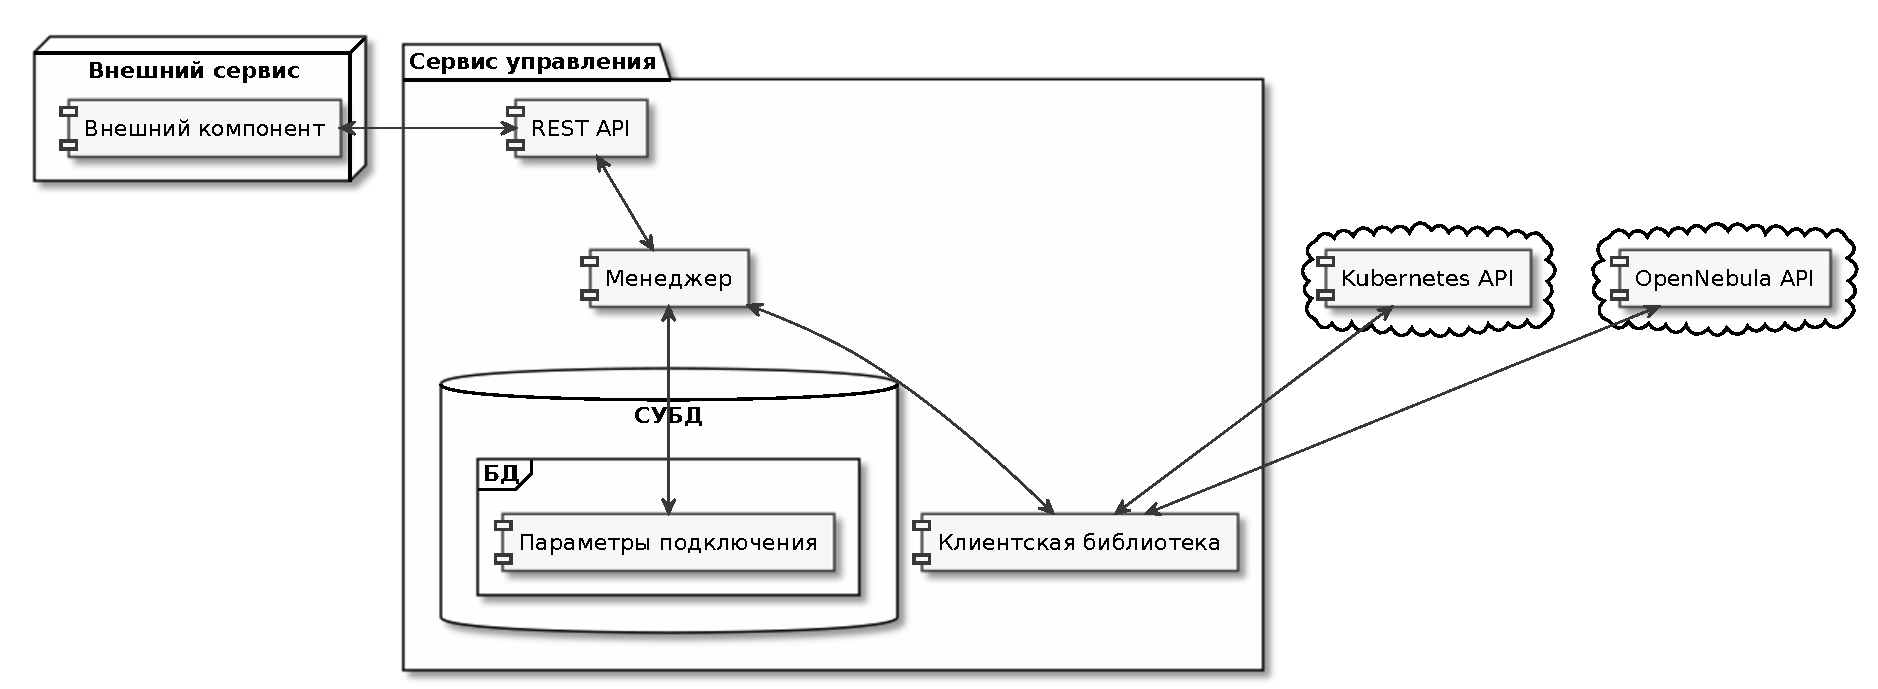
\includegraphics[width=\textwidth]{img/approach-organization.pdf}
    \caption{Предложенная организация решения}
    \label{approach-organization}
\end{figure}

\begin{figure}[hbtp]
    \centering
    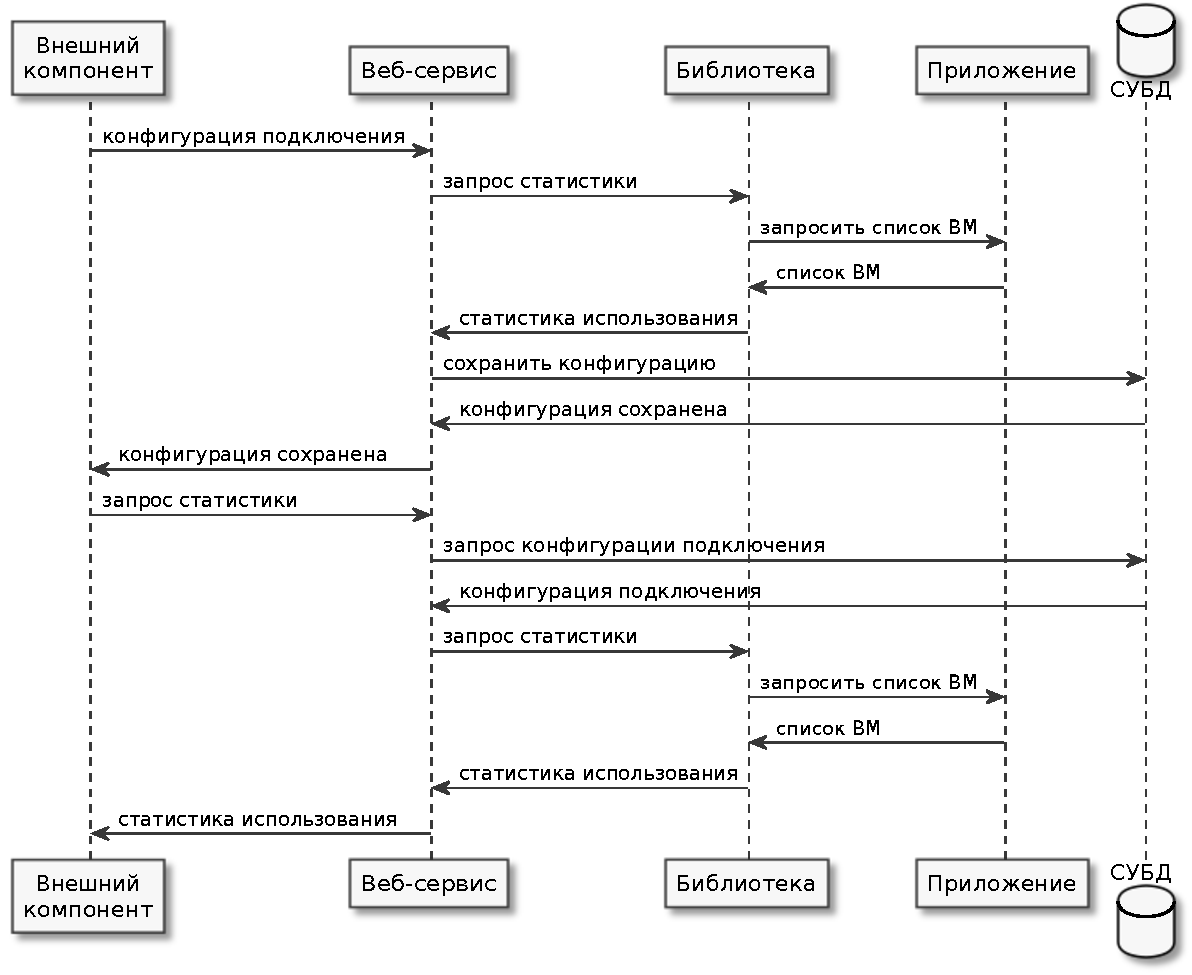
\includegraphics[width=\textwidth]{img/architecture-sequence.pdf}
    \caption{Диаграмма последовательности взаимодействия компонентов}
    \label{architecture-sequence}
\end{figure}
